
\chapter*{M4: Core-Local Message Passing}{\textbf{Author: Shane Nelson}
\newline 
 \newline 
 The goal of this milestone is to enable threads to access services such as process management and memory
 allocation via intra-core remote procedure calls.}
\addcontentsline{toc}{chapter}{M4: Core-Local Message Passing (LMP)}

\section{Architecture Overview}
Our M4 architecture is split cleanly between our client side request API contained in \newline \co{include/aos/aos_rpc.h} and our
server side handlers contained in \co{usr/init/rpc_server.c}. This section will focus on only the content in these
files relevant for LMP, there are many additional details in the source for these files, but these pertain to M6 and as such
are not discussed here. Figure~\ref{fig:m4arch} below is a diagram illustrating the overall LMP subsystem architecture.
\begin{figure}[H]
    \centering
    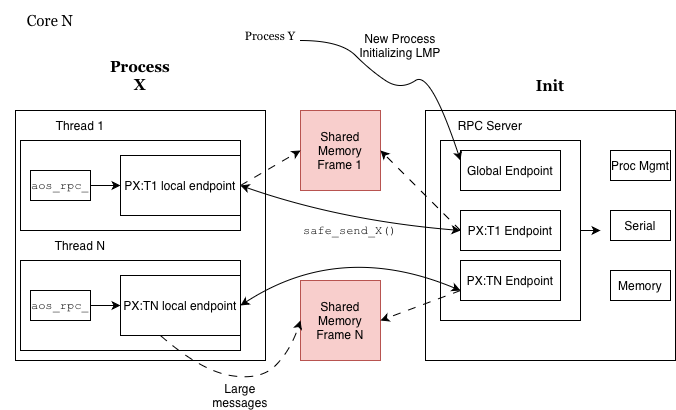
\includegraphics[width=1\textwidth]{images/finalm4.drawio.png}
    \caption{Overall LMP subsystem architecture.}
    \label{fig:m4arch}
\end{figure}
\subsection{Client-Side}
\label{sec:clientside}
We choose to implement per-thread lmp channels in order to increase the available concurrency in our system.
This allows any thread to wait on a process without blocking the progress of other threads, and a similar optimization
 was implemented by Linux (this behavior can be achieved by passing \co{__WNOTHREAD} to \co{waitid}). This also has the 
 benefit of making synchronization trivial but has the down-side of added initialization complexity.

\subsubsection{Thread-Local State}
Each thread keeps a \co{struct aos_rpc} which stores metadata about the channel, such as the channel itself and the
data pertaining to \hyperref[sec:shared_mem]{shared memory}. Each thread also keeps a distinct waitset which allows
the underlying system to correctly wakeup threads when messages have arrived on their channel. The exposed \co{get_X_channel()}
and \co{get_default_waitset()} functions are wired to use this thread-local state.

\subsubsection{Channel Initialization}
Each thread bootstraps its channel lazily on first use via a hook registered with the threading library.
The initialization follows a two-step handshake. First the thread creates a temporary \co{lmp_chan} aimed at
\co{cap_initep}, init's well-known global endpoint, creates a new local endpoint, and sends an \co{AOS_RPC_MSG_HANDSHAKE} message carrying
its own local endpoint capability. Init responds by allocating a dedicated per-thread channel and replying with
that channel's endpoint capability. The thread then replaces its \co{remote_cap} with this new per-thread endpoint,
and all subsequent communication bypasses the global endpoint entirely.

\subsubsection{Synchronous Send/Receive}
All RPCs follow a strict synchronous pattern, the client sends a tagged message via \co{safe_sendN()} (a \co{lmp_chan_send()} wrapper which transparently retries on a transient error), then
blocks on \co{recv_msg()} until a reply arrives. \co{recv_msg()} registers a one-shot callback on the
thread's private waitset and spins on \co{event_dispatch()} until the callback fires and marks the slot
as done. Because each thread has its own waitset and dedicated channel, threads never race to receive each
other's replies.

\subsection{Server-Side}
In order to facilitate per-thread channels our server maintains multiple LMP endpoints. One endpoint is a dedicated
global listening endpoint which handles the initialization of new channels. The server also maintains one endpoint per
user process thread, created after handshaking.

\subsubsection{Handshake Protocol}
Client processes are initialized with a capability \co{cap_selfep} when they are initially dispatched. This capability
points to the global endpoint. The client mints a new endpoint and sends it to init over the listening channel. This channel
is set up to only enter in \co{init_handshake_handler}. Once in the handler the server allocates a new local endpoint
to communicate with the child using the endpoint it receives, creates an lmp channel out of it and then sends this newly created endpoint back to the client
in a \co{AOS_RPC_MSG_ACK} tagged message. The server then creates a \co{struct client_state} which stores the per-client metadata
 such as the \co{lmp_chan} and information pertaining to the shared memory frame used for large messages. Finally the server registers another function \co{init_recv_handler} (the general purpose entry)
as the entry point for the newly created endpoint, and provides a closure with the created \co{struct client_state}. Now both sides can communicate on the dedicated channel.

\subsubsection{General Purpose Serving}
When a message is received on a dedicated channel, the system calls \co{init_recv_handler} and provides the closure created in the handshake. This function
reads the message type from the first byte of the message and calls the correct handler for the desired request type. The handler which is called is determined
using a table mapping message types (defined in \co{aos_rpc.h}) to function pointers. Once in the handler, the server will execute the desired command
locally, and send the client back either an acknowledgement message or the result of the RPC.

\subsubsection{Special Case: \co{aos_rpc_proc_wait()}}
When a thread wants to wait on a process, it must be notified via RPC when the process exits. To facilitate this, the process management function \co{prod_mgmt_register_wait()} maintains a linked list of \co{struct waiter_node}
 for each process which holds metadata about the client channel. When a client calls the wait rpc function, its channel is added to this list and it is not
sent a response. This blocks the thread because it is waiting in a synchronous receive loop which blocks it until
a message is received on the channel. When another thread (or \co{libc_exit}) terminates the waitee process, \co{proc_mgmt_terminated} is called.
This function walks the process's \co{waiter_node} linked list and sends an rpc message to the channel stored therein.
 This brings the thread out of its receive loop and unblocks it.


\subsection{Shared Memory for Large Messages}
\label{sec:shared_mem}
In order to reduce the latency for large messages, we implement a shared memory frame to pass such messages. Without shared memory
 we would be forced to break large messages into cacheline-sized messages and send them one by one. This likely has large
 latency implications (although we did not explore testing this). To implement this lazily, before a client sends a request which
 requires more than one cacheline it undergoes a shared memory handshake process with init as follows:
 \begin{enumerate}
    \item Client tries to request an operation that requires a request or response larger than one cacheline and sees that \co{struct aos_rpc.shm_vaddr} is NULL.
    \item Client allocates a physical memory frame.
    \item Client maps this frame into its virtual memory space and updates the \newline \co{struct aos_rpc.shm_vaddr} and \co{struct aos_rpc.shm_size} fields.
    \item Client sends frame capability to init in a \co{SHMEM_SETUP} message.
    \item Init maps the capability into its virtual address space and updates the corresponding \co{struct client_state} fields for the client.
    \item Init sends back a \co{SHMEM_ACK} message.
    \item Client proceeds to whichever operation was in progress.
 \end{enumerate}

\section{Optimizations and Performance Evaluation}
\subsection{Performance Goals and Optimizations}
Our performance goals for our optimizations of milestone 4 were (1) reduce the latency of multithreaded RPC, 
and (2) reduce the memory usage of our shared-memory approach.
\subsubsection{1. Latency Reduction for Multithreaded LMP}
We anticipate multithreaded workloads that make heavy usage of the local RPC infrastructure to perform
very poorly using a naive mutual-exclusion locking based approach to synchronization. For this reason we
introduced per-thread LMP channels which allows for greater concurrency in the face of load. The implementation
of this design is already discussed at length above, see \hyperref[sec:clientside]{Client-Side} for details. We test
the efficacy of this optimization below, see \hyperref[sec:performance-opt]{Performance Optimization}.
\subsubsection{2. Memory Usage Reduction of Large Message Infrastructure}
One of the main drawbacks of the prior optimization is the memory usage due to each channel having a frame allocated for shared memory communication. 
This memory usage obviously increases when the number of channels increases, as it does in our prior optimization from one per process
to one per thread. In a commercial system running many thousands of user-level threads, this presents a serious problem. To get around this
we lazily allocate shared memory frames only when an operation that needs a large message cannot fit the message in a certain (tunable) number 
of cachelines. This means that only a small subset of threads (those using RPC to pass large strings or those calling "ps" frequently) ever get
a shared physical memory frame allocated. Some further optimizations would be to intelligently deallocate frames when not in use, perhaps
using a variant of our \co{aos_rpc} API which tells the system to reclaim the frame after receipt of the data, and to make a variant
of the API which allows the system to run in "memory-constrained" mode which will opt to send cachelines message by message rather than
using any shared memory. We do not implement these optimizations, and importantly, due to time have not implemented memory-usage benchmarking
to judge the performance of the optimization we did implement.

\subsection{Performance Evaluation}
\label{sec:performance-opt}
\subsubsection{Microbenchmarks}
To facilitate comparing a non-optimized LMP implementation to our optimized implementation, we created 
three microbenchmarks:
\begin{description}
    \item \textbf{1. RTT: Round Trip Time.}
    
    This benchmark is designed to test the round trip cycle latency for a simple \newline \co{aos_rpc_send_number()} operation. It is single threaded and is initially run 20 times to warm up microarchitectural structures, then 200 times each collecting a cycle latency measurement.

    \item \textbf{2. Stress: Shared Memory RPC Stress Test.}
    
    This benchmark measures RPC latency under high multithreaded contention. 16 worker threads are spawned, they each run a warm-up phase, then all at once they each try to execute 50 \co{aos_rpc_send_string} operations, recording the latency of each operation. Thus we measure how LMP and our shared memory approach scale under high load.

    \item \textbf{3. MTW: MultiThreaded Wait.}
    
    This benchmark evaluates the effect of a long-lived blocking RPC on the throughput of concurrent RPC activity. Four worker threads simultaneously send various \co{aos_rpc} requests to init. When run in waiting mode, another thread first waits on a separate process, then the worker threads begin. When run in baseline mode, no such waiter exists. We expect our per-thread LMP implementation to see almost no drop off between modes, while the latency of the naive implementation should be bounded by the latency of the waitee process.
\end{description}
\subsubsection{Results}

We see a modest improvement in median Stress, insignificant difference in RTT, and as expected massive wins in MTW.
Figure~\ref{fig:bench-naive} displays the Stress and RTT results for the un-optimized build and Figure~\ref{fig:bench-perthread} displays the same results for our 
optimized build. RTT shows a significant increase in mean cycles, however this is swayed by a few outliers that are observed 
consistently at the end of the benchmark. Median (P50) RTT results show a slight increase for our optimized build. I believe this
to be due to a slight reduction in cacheability of perthread \co{struct aos_rpc} compared to per-process (although this is merely a hypothesis). 
Interestingly, the RTT distribution for the optimized group is consistently bimodal. We observe a periodic doubling in 
latency for single-threaded operations, and at present we cannot explain this phenomenon, this is an important area for 
future investigation.
 \newline
 \newline
Our multithreaded stress
test (Figures~\ref{fig:bench-naive}~\&~\ref{fig:bench-perthread} right panel) shows that our optimized build required at mean only 78\% as many cycles as the unoptimized build, and at median only 89\% of cycles.
Of importance is also the behavior of the tails where the unoptimized build had a significant number of latencies 2x 
higher than the maximum optimized latency. This explains the mean-median discrepancy. We find this to be the strongest result
for our implementation as multithreaded IPC-heavy workloads are readily imaginable.
 \newline
  \newline
 Finally, the results for our multithreaded waiter benchmark (Figure~\ref{fig:bench-mtw}) reflect our initial expectations exactly. Our optimized build saw only
a 26\% increase in latency with a blocked waiter, while the naive build saw a > 1000\% gain in latency, bounded by the time-to-exit of the waitee process.
This result reflects our initial motivation for building this optimization. It may seem heavily cherry-picked, but you could 
imagine an application such as a shell having such behavior.

\begin{figure}[H]
    \centering
    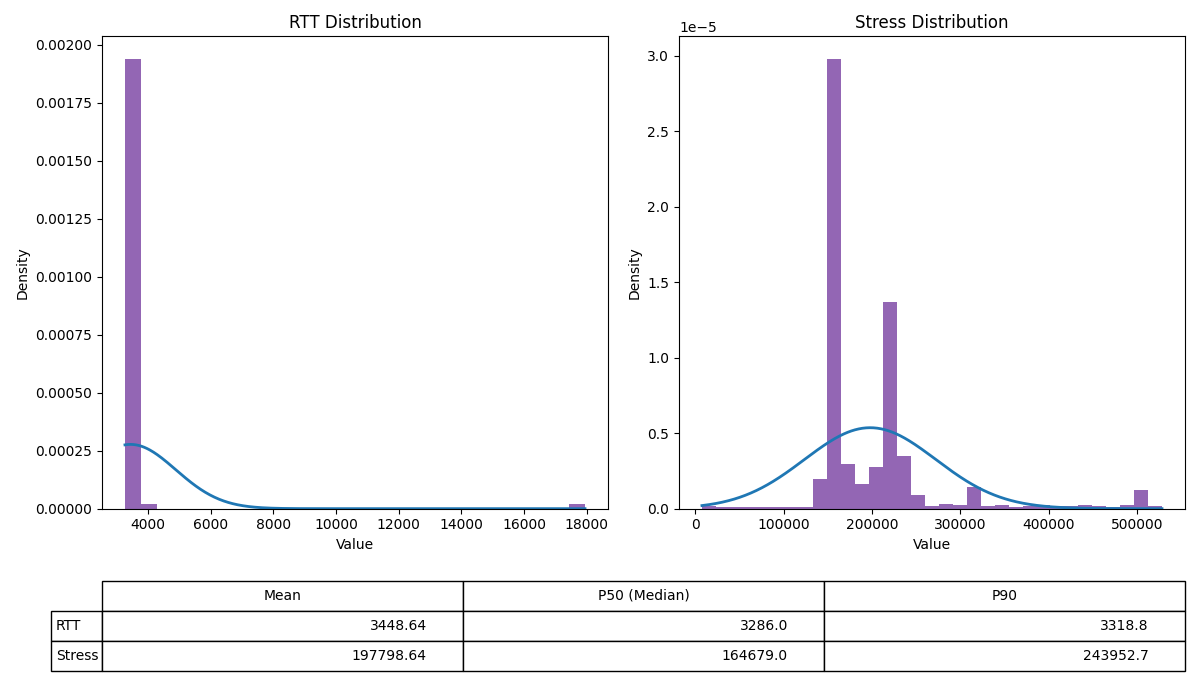
\includegraphics[width=1\textwidth]{images/naive_purple.png}
    \caption{Naive implementation benchmark results for a single-threaded number passing benchmark,
    labeled RTT, and a multithreaded string passing benchmark, labeled stress.}
    \label{fig:bench-naive}
\end{figure}

\begin{figure}[H]
    \centering
    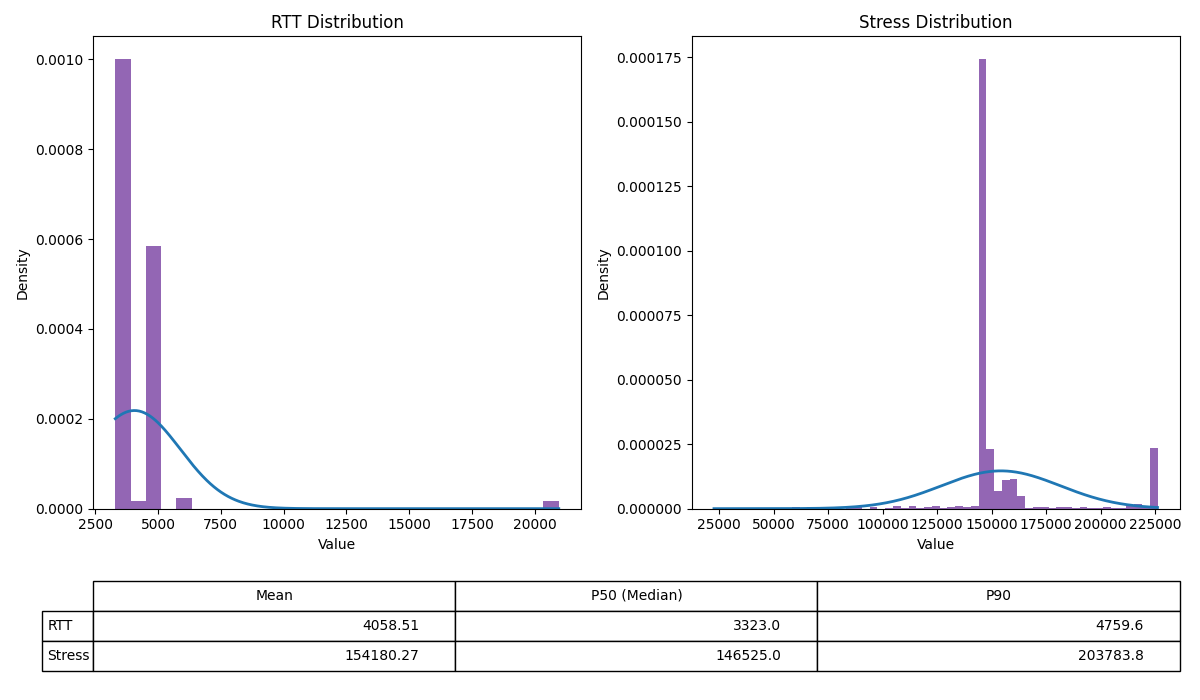
\includegraphics[width=1\textwidth]{images/perthread_purple.png}
    \caption{Per-thread implementation benchmark results for a single-threaded number passing benchmark,
    labeled RTT, and a multithreaded string passing benchmark, labeled stress. As can be seen the overhead to
    create a perthread channel (evident in the median RTT statistic) is negligible compared to the baseline. The per-thread implementation
    sees significant gains in median multithreaded latency.}
    \label{fig:bench-perthread}
\end{figure}

\begin{figure}[H]
    \centering
    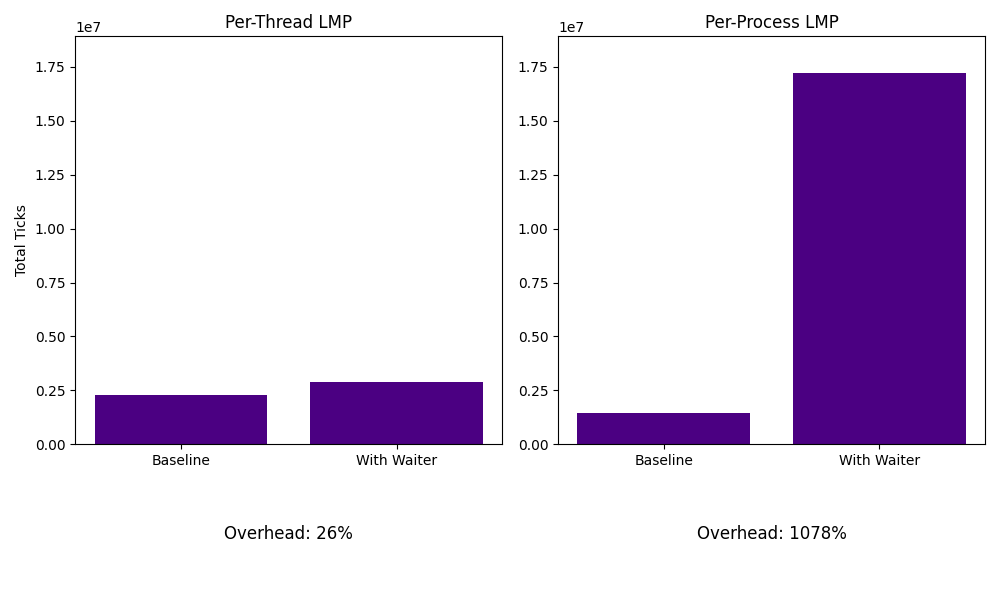
\includegraphics[width=1\textwidth]{images/waiting.png}
    \caption{Performance drop-off from running a multithreaded workload (MTW) without a
    thread waiting on a process to finish, to running one with a thread waiting. Per process lmp channels perform > 1000\%
    worse while a thread is waiting, whereas per-thread channels see only a modest 26\% cycle gain.}
    \label{fig:bench-mtw}
\end{figure}

\section{Development Process}
What I will call phase 1 began with Sahil writing the client side state and handlers in  \newline \co{aos_rpc.c}/\co{aos_rpc.h} as well as the original
initialization code in \co{barrelfish_initonthread()}. Allan then wrote the serverside entry point as well as
wrappers for all of the per-request handlers and the implementations of the memory and serial services. Shane then
finished the naive implementation by finishing the initialization, server, and client functionality, and implementing 
naive mutex-based synchronization and shared memory for large messages. At this point we were passing all of the \co{m4_grading} tests.
 \newline
 \newline
Phase 2 began after a conversation on Ed with Simon which motivated Shane to implement the optimizations above. This
involved reworking and hardening the implementation in phase 1, as well as changing the protocol to handle
 per-thread LMP channels. This required touching every LMP-related file as well as the threading library and was difficult to
 get running, requiring debugging with Simon in office hours. Using AI tooling
 tests were written for the optimization, which it passed.
 \newline
 \newline
 The final phase began when collecting data for this report, where Shane (with the help of AI tooling) reverted
 to an unoptimized version of the code. Shane then implemented 3 benchmarks, collected results, and wrote the M4 section
 of the report.
\newpage